\documentclass{standalone}
\usepackage{tikz}
\usetikzlibrary{patterns, positioning}

\begin{document}
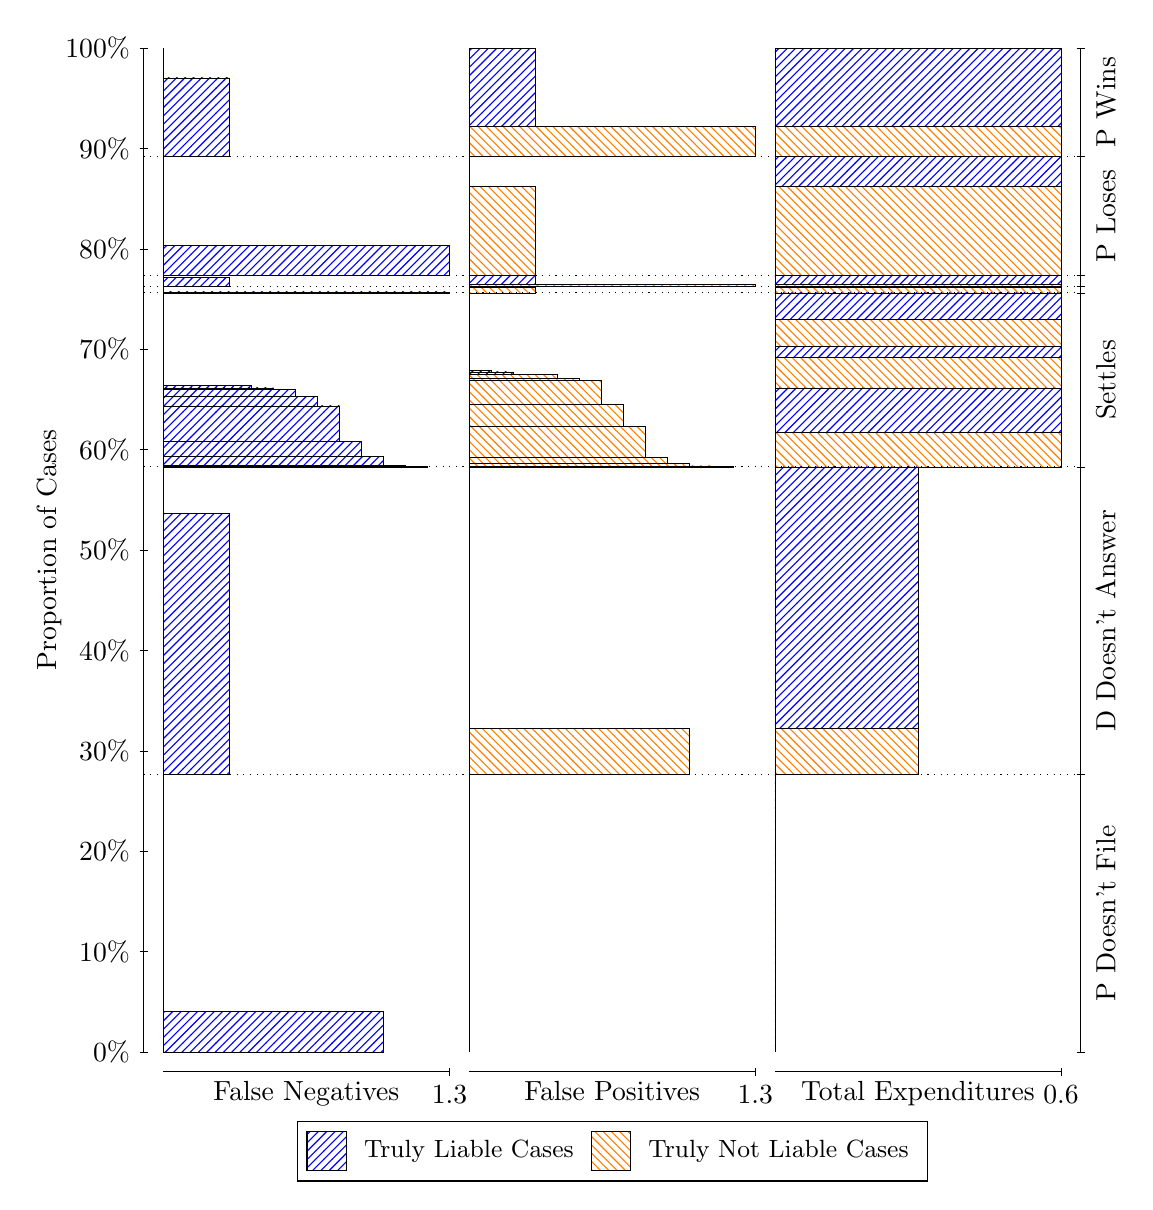
\begin{tikzpicture}
\draw[black, very thin] (1.5,1.75) -- (1.5,14.5);
\node[rotate=90, anchor=center] at (0.3, 8.125) {Proportion of Cases};
\draw[black, very thin] (1.45,1.75) -- (1.55,1.75);
\node[anchor=east] at (1.45, 1.75) {0\%};
\draw[black, very thin] (1.45,3.025) -- (1.55,3.025);
\node[anchor=east] at (1.45, 3.025) {10\%};
\draw[black, very thin] (1.45,4.3) -- (1.55,4.3);
\node[anchor=east] at (1.45, 4.3) {20\%};
\draw[black, very thin] (1.45,5.575) -- (1.55,5.575);
\node[anchor=east] at (1.45, 5.575) {30\%};
\draw[black, very thin] (1.45,6.85) -- (1.55,6.85);
\node[anchor=east] at (1.45, 6.85) {40\%};
\draw[black, very thin] (1.45,8.125) -- (1.55,8.125);
\node[anchor=east] at (1.45, 8.125) {50\%};
\draw[black, very thin] (1.45,9.4) -- (1.55,9.4);
\node[anchor=east] at (1.45, 9.4) {60\%};
\draw[black, very thin] (1.45,10.675) -- (1.55,10.675);
\node[anchor=east] at (1.45, 10.675) {70\%};
\draw[black, very thin] (1.45,11.95) -- (1.55,11.95);
\node[anchor=east] at (1.45, 11.95) {80\%};
\draw[black, very thin] (1.45,13.225) -- (1.55,13.225);
\node[anchor=east] at (1.45, 13.225) {90\%};
\draw[black, very thin] (1.45,14.5) -- (1.55,14.5);
\node[anchor=east] at (1.45, 14.5) {100\%};

\draw[black, very thin] (13.4,1.75) -- (13.4,14.5);
\draw[black, very thin] (13.35,1.75) -- (13.45,1.75);
\node[anchor=west] at (13.35, 1.75) {};
\draw[black, very thin] (13.35,5.2713) -- (13.45,5.2713);
\node[anchor=west] at (13.35, 5.2713) {};
\draw[black, very thin] (13.35,9.181) -- (13.45,9.181);
\node[anchor=west] at (13.35, 9.181) {};
\draw[black, very thin] (13.35,11.39) -- (13.45,11.39);
\node[anchor=west] at (13.35, 11.39) {};
\draw[black, very thin] (13.35,11.472) -- (13.45,11.472);
\node[anchor=west] at (13.35, 11.472) {};
\draw[black, very thin] (13.35,11.612) -- (13.45,11.612);
\node[anchor=west] at (13.35, 11.612) {};
\draw[black, very thin] (13.35,13.125) -- (13.45,13.125);
\node[anchor=west] at (13.35, 13.125) {};
\draw[black, very thin] (13.35,14.5) -- (13.45,14.5);
\node[anchor=west] at (13.35, 14.5) {};

\draw[black, very thin, pattern color=blue, pattern=north east lines] (1.75,1.75) rectangle (4.5449,2.2647);
\draw[black, very thin, pattern color=orange, pattern=north west lines] (1.75,2.2647) rectangle (1.75,5.2713);
\draw[black, very thin, pattern color=blue, pattern=north east lines] (1.75,5.2713) rectangle (2.5885,8.5935);
\draw[black, very thin, pattern color=orange, pattern=north west lines] (1.75,8.5935) rectangle (1.75,9.181);
\draw[black, very thin, pattern color=blue, pattern=north east lines] (1.75,9.181) rectangle (5.1038,9.1873);
\draw[black, very thin, pattern color=blue, pattern=north east lines] (1.75,9.1873) rectangle (4.8244,9.1949);
\draw[black, very thin, pattern color=blue, pattern=north east lines] (1.75,9.1949) rectangle (4.5449,9.3163);
\draw[black, very thin, pattern color=blue, pattern=north east lines] (1.75,9.3163) rectangle (4.2654,9.3184);
\draw[black, very thin, pattern color=blue, pattern=north east lines] (1.75,9.3184) rectangle (4.2654,9.5018);
\draw[black, very thin, pattern color=blue, pattern=north east lines] (1.75,9.5018) rectangle (3.9859,9.9552);
\draw[black, very thin, pattern color=blue, pattern=north east lines] (1.75,9.9552) rectangle (3.7064,10.074);
\draw[black, very thin, pattern color=blue, pattern=north east lines] (1.75,10.074) rectangle (3.4269,10.167);
\draw[black, very thin, pattern color=blue, pattern=north east lines] (1.75,10.167) rectangle (3.1474,10.185);
\draw[black, very thin, pattern color=blue, pattern=north east lines] (1.75,10.185) rectangle (2.8679,10.219);
\draw[black, very thin, pattern color=orange, pattern=north west lines] (1.75,10.219) rectangle (1.75,11.39);
\draw[black, very thin, pattern color=blue, pattern=north east lines] (1.75,11.39) rectangle (5.3833,11.404);
\draw[black, very thin, pattern color=orange, pattern=north west lines] (1.75,11.404) rectangle (1.75,11.472);
\draw[black, very thin, pattern color=blue, pattern=north east lines] (1.75,11.472) rectangle (2.5885,11.583);
\draw[black, very thin, pattern color=orange, pattern=north west lines] (1.75,11.583) rectangle (1.75,11.612);
\draw[black, very thin, pattern color=blue, pattern=north east lines] (1.75,11.612) rectangle (5.3833,11.99);
\draw[black, very thin, pattern color=orange, pattern=north west lines] (1.75,11.99) rectangle (1.75,13.125);
\draw[black, very thin, pattern color=blue, pattern=north east lines] (1.75,13.125) rectangle (2.5885,14.122);
\draw[black, very thin, pattern color=orange, pattern=north west lines] (1.75,14.122) rectangle (1.75,14.5);
\draw[black, very thin, pattern color=orange, pattern=north west lines] (5.6333,1.75) rectangle (5.6333,4.7566);
\draw[black, very thin, pattern color=blue, pattern=north east lines] (5.6333,4.7566) rectangle (5.6333,5.2713);
\draw[black, very thin, pattern color=orange, pattern=north west lines] (5.6333,5.2713) rectangle (8.4282,5.8588);
\draw[black, very thin, pattern color=blue, pattern=north east lines] (5.6333,5.8588) rectangle (5.6333,9.181);
\draw[black, very thin, pattern color=orange, pattern=north west lines] (5.6333,9.181) rectangle (8.9872,9.1865);
\draw[black, very thin, pattern color=orange, pattern=north west lines] (5.6333,9.1865) rectangle (8.7077,9.1919);
\draw[black, very thin, pattern color=orange, pattern=north west lines] (5.6333,9.1919) rectangle (8.4282,9.2291);
\draw[black, very thin, pattern color=orange, pattern=north west lines] (5.6333,9.2291) rectangle (8.1487,9.2981);
\draw[black, very thin, pattern color=orange, pattern=north west lines] (5.6333,9.2981) rectangle (7.8692,9.6945);
\draw[black, very thin, pattern color=orange, pattern=north west lines] (5.6333,9.6945) rectangle (7.5897,9.9706);
\draw[black, very thin, pattern color=orange, pattern=north west lines] (5.6333,9.9706) rectangle (7.3103,10.275);
\draw[black, very thin, pattern color=orange, pattern=north west lines] (5.6333,10.275) rectangle (7.0308,10.308);
\draw[black, very thin, pattern color=orange, pattern=north west lines] (5.6333,10.308) rectangle (6.7513,10.353);
\draw[black, very thin, pattern color=blue, pattern=north east lines] (5.6333,10.353) rectangle (6.1923,10.387);
\draw[black, very thin, pattern color=blue, pattern=north east lines] (5.6333,10.387) rectangle (5.9128,10.405);
\draw[black, very thin, pattern color=blue, pattern=north east lines] (5.6333,10.405) rectangle (5.6333,11.39);
\draw[black, very thin, pattern color=orange, pattern=north west lines] (5.6333,11.39) rectangle (6.4718,11.458);
\draw[black, very thin, pattern color=blue, pattern=north east lines] (5.6333,11.458) rectangle (5.6333,11.472);
\draw[black, very thin, pattern color=orange, pattern=north west lines] (5.6333,11.472) rectangle (9.2667,11.501);
\draw[black, very thin, pattern color=blue, pattern=north east lines] (5.6333,11.501) rectangle (6.4718,11.612);
\draw[black, very thin, pattern color=orange, pattern=north west lines] (5.6333,11.612) rectangle (6.4718,12.747);
\draw[black, very thin, pattern color=blue, pattern=north east lines] (5.6333,12.747) rectangle (5.6333,13.125);
\draw[black, very thin, pattern color=orange, pattern=north west lines] (5.6333,13.125) rectangle (9.2667,13.503);
\draw[black, very thin, pattern color=blue, pattern=north east lines] (5.6333,13.503) rectangle (6.4718,14.5);
\draw[black, very thin, pattern color=orange, pattern=north west lines] (9.5167,1.75) rectangle (9.5167,4.7566);
\draw[black, very thin, pattern color=blue, pattern=north east lines] (9.5167,4.7566) rectangle (9.5167,5.2713);
\draw[black, very thin, pattern color=orange, pattern=north west lines] (9.5167,5.2713) rectangle (11.333,5.8588);
\draw[black, very thin, pattern color=blue, pattern=north east lines] (9.5167,5.8588) rectangle (11.333,9.181);
\draw[black, very thin, pattern color=orange, pattern=north west lines] (9.5167,9.181) rectangle (13.15,9.62);
\draw[black, very thin, pattern color=blue, pattern=north east lines] (9.5167,9.62) rectangle (13.15,10.184);
\draw[black, very thin, pattern color=orange, pattern=north west lines] (9.5167,10.184) rectangle (13.15,10.57);
\draw[black, very thin, pattern color=blue, pattern=north east lines] (9.5167,10.57) rectangle (13.15,10.708);
\draw[black, very thin, pattern color=orange, pattern=north west lines] (9.5167,10.708) rectangle (13.15,11.054);
\draw[black, very thin, pattern color=blue, pattern=north east lines] (9.5167,11.054) rectangle (13.15,11.39);
\draw[black, very thin, pattern color=orange, pattern=north west lines] (9.5167,11.39) rectangle (13.15,11.458);
\draw[black, very thin, pattern color=blue, pattern=north east lines] (9.5167,11.458) rectangle (13.15,11.472);
\draw[black, very thin, pattern color=orange, pattern=north west lines] (9.5167,11.472) rectangle (13.15,11.501);
\draw[black, very thin, pattern color=blue, pattern=north east lines] (9.5167,11.501) rectangle (13.15,11.612);
\draw[black, very thin, pattern color=orange, pattern=north west lines] (9.5167,11.612) rectangle (13.15,12.747);
\draw[black, very thin, pattern color=blue, pattern=north east lines] (9.5167,12.747) rectangle (13.15,13.125);
\draw[black, very thin, pattern color=orange, pattern=north west lines] (9.5167,13.125) rectangle (13.15,13.503);
\draw[black, very thin, pattern color=blue, pattern=north east lines] (9.5167,13.503) rectangle (13.15,14.5);
\draw[black, dotted] (1.5,5.2713) -- (13.4,5.2713);
\draw[black, dotted] (1.5,9.181) -- (13.4,9.181);
\draw[black, dotted] (1.5,11.39) -- (13.4,11.39);
\draw[black, dotted] (1.5,11.472) -- (13.4,11.472);
\draw[black, dotted] (1.5,11.612) -- (13.4,11.612);
\draw[black, dotted] (1.5,13.125) -- (13.4,13.125);
\draw[black, very thin] (1.75,1.5) -- (5.3833,1.5);
\node[anchor=north] at (3.5667, 1.5) {False Negatives};
\draw[black, very thin] (5.3833,1.45) -- (5.3833,1.55);
\node[anchor=north] at (5.3833, 1.45) {1.3};

\draw[black, very thin] (5.6333,1.5) -- (9.2667,1.5);
\node[anchor=north] at (7.45, 1.5) {False Positives};
\draw[black, very thin] (9.2667,1.45) -- (9.2667,1.55);
\node[anchor=north] at (9.2667, 1.45) {1.3};

\draw[black, very thin] (9.5167,1.5) -- (13.15,1.5);
\node[anchor=north] at (11.333, 1.5) {Total Expenditures};
\draw[black, very thin] (13.15,1.45) -- (13.15,1.55);
\node[anchor=north] at (13.15, 1.45) {0.6};

\node[black, centered, rotate=90] at (13.72, 3.5106) {P Doesn't File};
\node[black, centered, rotate=90] at (13.72, 7.2262) {D Doesn't Answer};
\node[black, centered, rotate=90] at (13.72, 10.286) {Settles};


\node[black, centered, rotate=90] at (13.72, 12.369) {P Loses};
\node[black, centered, rotate=90] at (13.72, 13.813) {P Wins};

\draw (7.449999999999999,1.5) node[draw=none] (baseCoordinate) {};
\begin{scope}[align=center]
        \matrix[scale=0.5, draw=black, below=0.5cm of baseCoordinate, nodes={draw}, column sep=0.1cm]{
            \node[rectangle, draw, minimum width=0.5cm, minimum height=0.5cm, pattern=north east lines, pattern color=blue] {}; &
            \node[draw=none, font=\small] (B) {Truly Liable Cases}; &
            \node[rectangle, draw, minimum width=0.5cm, minimum height=0.5cm, pattern=north west lines, pattern color=orange] {}; &
            \node[draw=none, font=\small] (B) {Truly Not Liable Cases}; \\
            };
\end{scope}

\end{tikzpicture}
\end{document}